\documentclass{article}
\usepackage[utf8]{inputenc}

%% Language and font encodings
\usepackage[english]{babel}
% \usepackage[utf8x]{inputenc}
\usepackage[T1]{fontenc}

%% Sets page size and margins
\usepackage[a4paper,top=2cm,bottom=2cm,left=2cm,right=2cm,marginparwidth=2cm]{geometry}

% %% for tabbing figures
% \usepackage{cuted}%%\stripsep-3pt
\usepackage{caption}
\usepackage{grffile}	% handle multi suffix (.drawio.png)
\usepackage{graphicx}
\usepackage{subfigure}  % multi-pictures in the same line

%% Sets row spaces
\usepackage{setspace}
\renewcommand{\baselinestretch}{1.0}

%% packages for tables
\usepackage{booktabs}

%% packages for tables
\usepackage{booktabs}

%% packages for code
\usepackage{xcolor}
\usepackage{listings}
\newcommand*{\listingautorefname}{Code}
\lstset{
	showstringspaces=false, %不显示中间的空格
}
\lstdefinestyle{lfonts}{
	basicstyle = \normalsize\ttfamily,
	stringstyle = \color{purple},
	keywordstyle = \color{blue!60!black}\bfseries,
	commentstyle = \color{olive}\scshape,
}
\lstdefinestyle{lnumbers}{
	numbers = left,
	numberstyle = \tiny,
	numbersep = 1em,
	firstnumber = 1,
	stepnumber = 1,
}
\lstdefinestyle{llayout}{
	breaklines = true,
	tabsize = 2,
	columns = flexible,
}
\lstdefinestyle{lgeometry}{
	xleftmargin = 20pt,
	xrightmargin = 0pt,
	frame = tb,
	framesep = \fboxsep,
	framexleftmargin = 20pt,
}
\lstdefinestyle{lgeneral}{
	style = lfonts,
	style = lnumbers,
	style = llayout,
	style = lgeometry,
}
\lstdefinestyle{python}{
	language = {Python},
	style = lgeneral,
}
\lstdefinestyle{shell}{
	language = {Shell},
	style = lgeneral,
}

%% packages for pseudocode
\usepackage{algorithm}
\usepackage{algorithmicx}  
\usepackage{algpseudocode}
\usepackage{amsmath}

%% packages for appendix
\usepackage[toc,page]{appendix}
\newcommand*{\Appendixautorefname}{Appendix}

%% Useful packages
\usepackage{amsmath}
\usepackage{graphicx}
\usepackage[colorinlistoftodos]{todonotes}
\usepackage[colorlinks=true, allcolors=blue]{hyperref}
\usepackage[numbers,sort&compress]{natbib} 
\usepackage{float}	% used for fix the location of tables and graphics
\usepackage{subfigure}  % multi-pictures in the same line
\newcommand{\upcite}[1]{\textsuperscript{\cite{#1}}}
\newcommand{\topcaption}{%
	\setlength{\abovecaptionskip}{0pt}%
	\setlength{\belowcaptionskip}{10pt}%
	\caption}

\title{\textbf{ECE329 Project \#2 Report}}
\author{Ruiqi Li, 3180111638}
\date{\today}

\begin{document}

%% for pseudo code
\renewcommand{\algorithmicrequire}{\textbf{Input:}}  % Use Input in the format of Algorithm
\renewcommand{\algorithmicensure}{\textbf{Output:}} % Use Output in the format of Algorithm
\newcommand{\algorithmautorefname}{Algorithm} % for hyperref

\maketitle

\section{Problem 1}

    \textbf{(20 pts) Please derive the analytical solution of $v(z, t)$ and $i(v, t)$ assuming $v_s(t) = V_0 sin(\omega t)$ so that you do not need to worry about the transient effects. Please show your derivation. } \\

    Since $\beta l = \beta d = \beta \frac{\lambda}{4} = \beta \frac{2\pi}{4\beta} = \frac{\pi}{2}$, we have.

    \begin{equation}
        \Gamma_L = \frac{Z_L - Z_c}{Z_L + Z_c} = \frac{25 - 50}{25 + 50} = -\frac{1}{3}
    \end{equation}

    Also, for $Z_{\text{in}}$ we compute it from the formula:

    \begin{equation}
        Z_{\text{in}} = Z(-d) = Z_C \frac{Z_L + jZ_C \tan{\beta d}}{Z_C + jZ_L \tan{\beta d}} = \frac{Z_C^2}{Z_L} = 100 \Omega
    \end{equation}

    Then, using KVL we have:

    \begin{equation}
        V(-d) = V_s \frac{Z_{\text{in}}}{Z_{\text{in}} + R_s} = \frac{1}{2}V_s = -j\frac{1}{2}V_0
    \end{equation}

    Substitute this value into $\tilde{V}(z) = \tilde{V}^+(e^{-j\beta z} + \Gamma_0 e^{j\beta z})$, we have that $\tilde{V}^+ = -\frac{3}{8}$. Similarly we can get the expression for current. Finally:

    \begin{align}
        \tilde{V}(z) &= -\frac{3}{8}e^{-j\beta z} + \frac{1}{8}e^{j\beta z} \nonumber \\
        \tilde{I}(z) &= -\frac{3}{400}e^{-j\beta z} - \frac{1}{400}e^{j\beta z} \nonumber
    \end{align}

    or, 

    \begin{align}
        v(z, t) &= -\frac{3}{8}\cos(\omega t - \beta z) + \frac{1}{8}\cos(\omega t + \beta z) \nonumber \\
        i(z, t) &= -\frac{3}{400}\cos(\omega t - \beta z) - \frac{1}{400}\cos(\omega t + \beta z) \nonumber
    \end{align}

\section{Problem 2}

    \textbf{Please find the load voltage $v_L(t) = v(z=0,t)$, for $0 \leq t \leq 10T$ using the 
    FDTD method given $v_S(t) = V_0sin(\omega t) u(t)$. }

    \subsection{(i)}

        To normalsize the results, assume that $T = 10$s and $\lambda = 4$m. Also, to help simplify the parameters, let $\Delta z_0 = \frac{1}{20}\lambda$ and $\Delta t_0 = \frac{\Delta z }{v_p}$. Here are the results of the simulations:

        \begin{itemize}
            \item[] For $\Delta z = 2 * \Delta z_0$ and $\Delta t = 2 * \Delta t_0$:
            
                \begin{figure}[H]
                    \centering
                    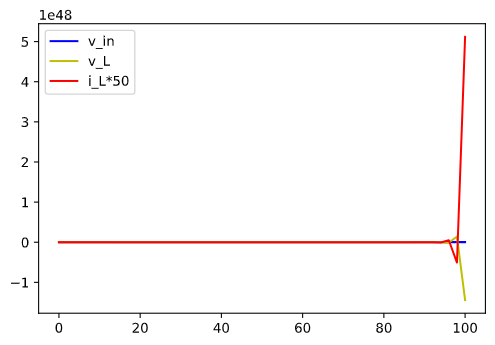
\includegraphics[width=0.5\textwidth]{img/2z0_2t0.png}
                    \caption{Plot for $\Delta z = 2 * \Delta z_0$ and $\Delta t = 2 * \Delta t_0$}
                    \label{fig:2z0-2t0}
                \end{figure}

            \item[] For $\Delta z = \Delta z_0$ and $\Delta t = \Delta t_0$: 
            
                \begin{figure}[H]
                    \centering
                    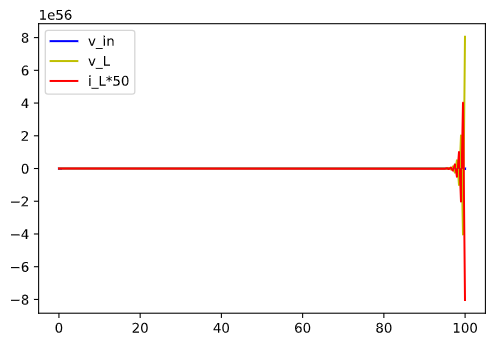
\includegraphics[width=0.5\textwidth]{img/z0_t0.png}
                    \caption{Plot for $\Delta z = \Delta z_0$ and $\Delta t = \Delta t_0$}
                    \label{fig:z0-t0}
                \end{figure}

            \item[] For $\Delta z = \frac{1}{2}\Delta z_0$ and $\Delta t = \Delta t_0$: 
            
                \begin{figure}[H]
                    \centering
                    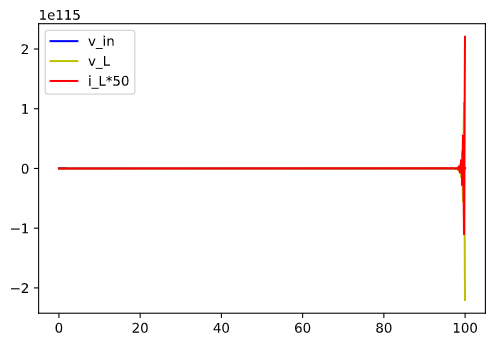
\includegraphics[width=0.5\textwidth]{img/z02_t0.png}
                    \caption{Plot for $\Delta z = \frac{1}{2}\Delta z_0$ and $\Delta t = \Delta t_0$}
                    \label{fig:z02-t0}
                \end{figure}

            \item[] For $\Delta z = \Delta z_0$ and $\Delta t = \frac{1}{2}\Delta t_0$: 
            
                \begin{figure}[H]
                    \centering
                    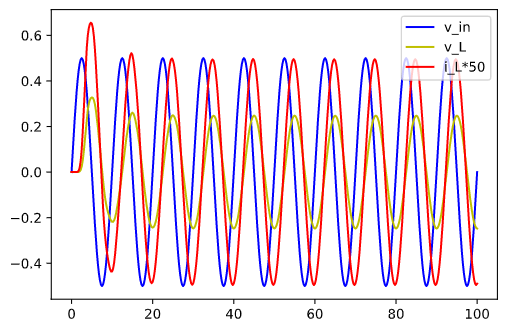
\includegraphics[width=0.5\textwidth]{img/z0_t02.png}
                    \caption{Plot for $\Delta z = \Delta z_0$ and $\Delta t = \frac{1}{2}\Delta t_0$}
                    \label{fig:z0-t02}
                \end{figure}

            \item[] For $\Delta z = \frac{1}{2}\Delta z_0$ and $\Delta t = \frac{1}{2}\Delta t_0$: 
            
                \begin{figure}[H]
                    \centering
                    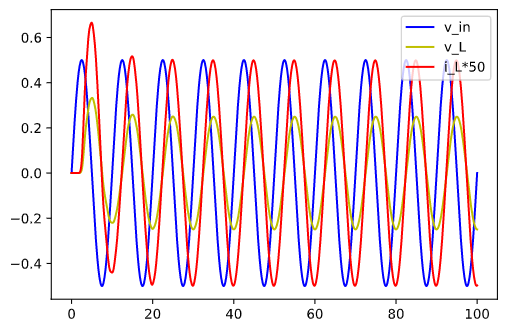
\includegraphics[width=0.5\textwidth]{img/z02_t02.png}
                    \caption{Plot for $\Delta z = \frac{1}{2}\Delta z_0$ and $\Delta t = \frac{1}{2}\Delta t_0$}
                    \label{fig:z02-t02}
                \end{figure}

            \item[] For $\Delta z = \frac{1}{5}\Delta z_0$ and $\Delta t = \frac{1}{5}\Delta t_0$: 
            
                \begin{figure}[H]
                    \centering
                    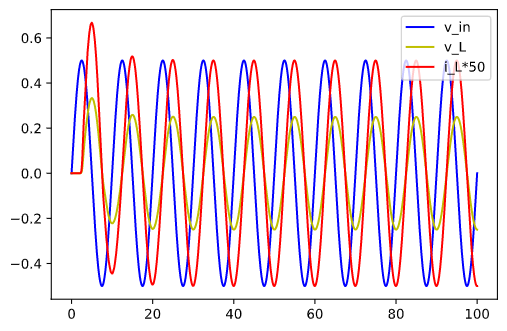
\includegraphics[width=0.5\textwidth]{img/z05_t05.png}
                    \caption{Plot for $\Delta z = \frac{1}{5}\Delta z_0$ and $\Delta t = \frac{1}{5}\Delta t_0$}
                    \label{fig:z05-t05}
                \end{figure}
        \end{itemize}

        From above we can see that as $\Delta z$ and $\Delta t$ decrease, the accuracy and stability both increase. Also, it seems that $\Delta t$ is more significant then $\Delta z$ when concerning stability. Considering accuracy, stability and efficiency, we choose $\Delta z = \frac{1}{2}\Delta z_0$ and $\Delta t = \frac{1}{2}\Delta t_0$. The comparison between the numerical results and the analytical results are shown below:

        \begin{figure}[H]
            \centering
            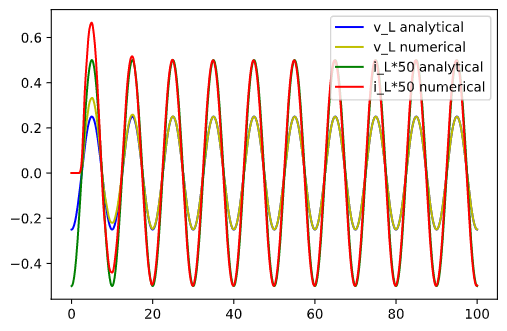
\includegraphics[width=0.5\textwidth]{img/2_1_comparison.png}
            \caption{Comparison between Numerical and Analytical Results using $\Delta z = \frac{1}{2}\Delta z_0$ and $\Delta t = \frac{1}{2}\Delta t_0$}
            \label{fig:2-1-comparison}
        \end{figure}

        It's obvious that they converge well after only about 1.5 cycles.

    \subsection{(ii)}

        The comparison result is shown as \autoref{fig:2-1-comparison}. The numerical solution converges well.

    \subsection{(iii)}

        If $d=0$, then $V_L(t) = V_s \frac{R_L}{R_L + R_s} = \frac{1}{5}\sin(\omega t)u(t)$, and $I_L(t) = \frac{V_L}{R_L} = \frac{1}{125}\sin(\omega t)u(t)$.

        \begin{figure}[H]
            \centering
            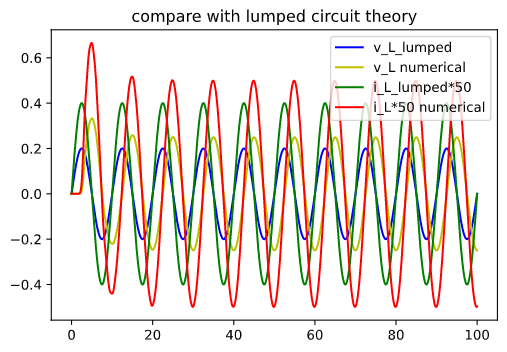
\includegraphics[width=0.5\textwidth]{img/2_3_comparison.png}
            \caption{Comparison between the Results with the Lumped Circuit Theory Results using $\Delta z = \frac{1}{2}\Delta z_0$ and $\Delta t = \frac{1}{2}\Delta t_0$}
            \label{fig:2-3-comparison}
        \end{figure}

        It shows that not only the amplitude is decreases from the lumped circuit theory results to the numerical results, the phase is also shifted.

\section{Problem 3}

    All the results are shown below:

    \begin{figure}[H]
        \centering
        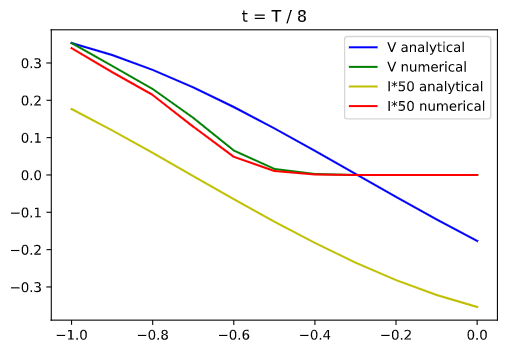
\includegraphics[width=0.5\textwidth]{img/3_1.png}
        \caption{Comparison between Numerical and Analytical with $t = \frac{T}{8}$}
        \label{fig:3-1}
    \end{figure}

    \begin{figure}[H]
        \centering
        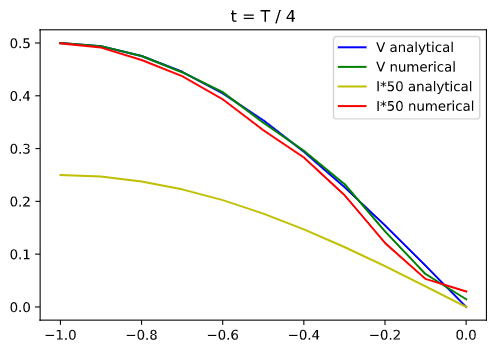
\includegraphics[width=0.5\textwidth]{img/3_2.png}
        \caption{Comparison between Numerical and Analytical with $t = \frac{T}{4}$}
        \label{fig:3-2}
    \end{figure}

    \begin{figure}[H]
        \centering
        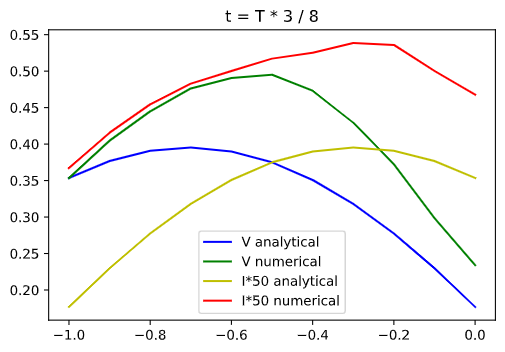
\includegraphics[width=0.5\textwidth]{img/3_3.png}
        \caption{Comparison between Numerical and Analytical with $t = \frac{3T}{8}$}
        \label{fig:3-3}
    \end{figure}

    \begin{figure}[H]
        \centering
        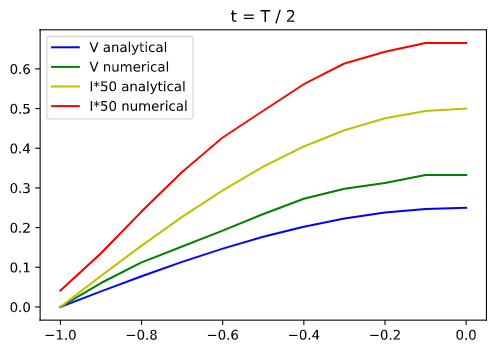
\includegraphics[width=0.5\textwidth]{img/3_4.png}
        \caption{Comparison between Numerical and Analytical with $t = \frac{T}{2}$}
        \label{fig:3-4}
    \end{figure}

    \begin{figure}[H]
        \centering
        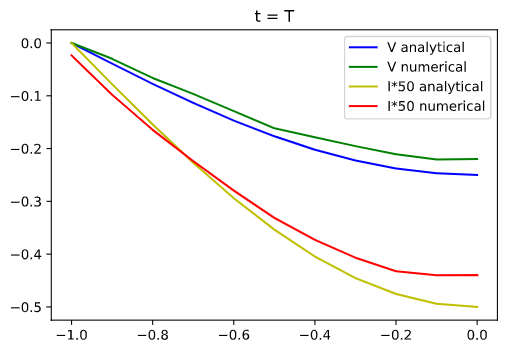
\includegraphics[width=0.5\textwidth]{img/3_5.png}
        \caption{Comparison between Numerical and Analytical with $t = T$}
        \label{fig:3-5}
    \end{figure}

    \begin{figure}[H]
        \centering
        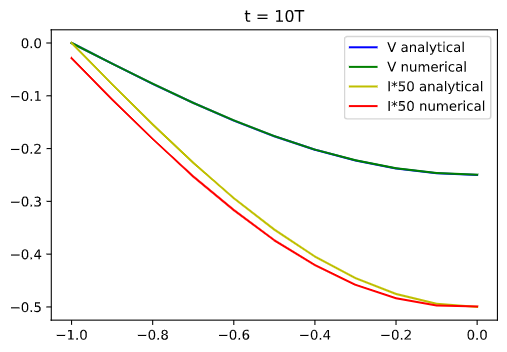
\includegraphics[width=0.5\textwidth]{img/3_6.png}
        \caption{Comparison between Numerical and Analytical with $t = 10T$}
        \label{fig:3-6}
    \end{figure}

    As shown above, it takes some time for the simulation to be stable. About 1 period is enough.

\end{document}
